\chapter{尤度場モデルを使用したパーティクルフィルタ}
\section{はじめに}
本章では, 尤度場モデルを使用したパーティクルフィルタについて説明をする. 
尤度場モデルを使用したパーティクルフィルタは, 手持ちの地図から事前に求めた, 
マップ上の障害物検知の尤度を表すxy座標上の関数をパーティクルの尤度計算に使用して
自己位置を推定するアルゴリズムである. 
この方法は, 得られるパーティクルの確率分布が雑然とした環境でも滑らかになることや尤度場の事前計算によって
計算効率の高いことがメリットとしてある. 

\section{パーティクルフィルタの目的・理論}

パーティクルフィルタは初期位置である$x_0$から、入力される情報、状態遷移モデル、観測モデルを使用することで、
確率密度関数である信念分布$b_t$を求め、パーティクルによる近似によって推定した自己位置である$x$を求めることを目的としている。
$x$は$\sum_{world}$上でのロボットの位置を(x, y),向きを$\theta$で表した、
式(\ref{exp:x})のようなロボットの姿勢である。

\begin{eqnarray}
  \label{exp:x}
  x = (x, y ,\theta)^T
\end{eqnarray}

\subsection{自己位置推定における信念分布}

最初の姿勢を$x_0$、これまでの制御指令値を式(\ref{exp:u})、センサ値を式(\ref{exp:z})とした場合、
推定したロボットの自己位置を表した信念分布$b_t$は式(\ref{exp:b_t})になる。

\begin{eqnarray}
  \label{exp:u}
  u_{1:t} = \{u_t|t=1,2,3,...,t\} 
\end{eqnarray}

\begin{eqnarray}
  \label{exp:z}
  z_{1:t} = \{z_t|t=1,2,3,...,t\} 
\end{eqnarray}

\begin{eqnarray}
  \label{exp:b_t}
  b_t(x) = p_t(x|x_0, u_{1:t}, z_{1:t}) 
\end{eqnarray}
式(\ref{exp:b_t})の右辺から信念分布$b_t$を求めるためには状態遷移モデルである式(\ref{exp:u_m})と
観測モデルである式(\ref{exp:z_m})を用いる。

\begin{eqnarray}
  \label{exp:u_m}
  x_t 〜 p(x|x_{t-1}, u_t)
\end{eqnarray}

\begin{eqnarray}
  \label{exp:z_m}
  z_t 〜 p(z|x_t)
\end{eqnarray}

\subsection{状態遷移モデルによる事前分布}

ロボットが時刻t-1からtまで、制御指令値である$u_t$によって移動した場合、
信念分布はロボットの姿勢と同様に$b_{t-1}$から遷移をする。
遷移後の信念分布は式(\ref{exp:b_hat})である$\hat{b_t}$として表される。

\begin{eqnarray}
  \label{exp:b_hat}
  \hat{b_t}(x) &=& p_t(x|x_0, u_{1:t}, z_{1:t-1}) \nonumber \\
  &=& \int_{x'\in\chi} p(x|x', u_t)b_{t-1}(x')dx' \nonumber \\
  &=& {<p(x|x', u_t)>}_{b_{t-1(x')}}
\end{eqnarray}

\subsection{観測更新による事後分布}

遷移後に観測$z_t$が得られた場合、ベイズの定理によって
信念分布$\hat{b_t}$の更新を行うことができる。
更新後の信念分布は式(\ref{exp:b_beizu})で表された$b_t$になる。

\begin{eqnarray}
  \label{exp:b_beizu}
  b_t(x) &=& \hat{b_t}(x|z_t) \nonumber \\
  &=& \frac{p(z_t|x)\hat{b_t}(x)}{p(z_t)} \nonumber \\
  &=& \eta p(z_t|x)\hat{b_t}(x)
\end{eqnarray}

\subsection{パーティクルによる近似}

信念分布$b_t$は$N$個のパーティクルによるパーティクルフィルタによって近似される。
近似された信念分布$b_t$は、式(\ref{exp:b_p})になる。

\begin{eqnarray}
  \label{exp:b_p}
  P(x*\in X) &=& \int_{x'\in\chi}b_t(x)dx \nonumber \\
  &\approx& \frac{1}{N} \sum_{i=0}^{N-1} \delta (x^{(i)}_{t} \in X)
\end{eqnarray}

そして、観測による更新を考慮すると、式(\ref{exp:b_p})は
重み$w_t$によって式(\ref{exp:b_p_z})になる。

\begin{eqnarray}
  \label{exp:b_p_z}
  P(x*\in X) &=& \int_{x'\in\chi}b_t(x)dx \nonumber \\
  &\approx& \sum_{i=0}^{N-1} w^{(i)}_{t} \delta (x^{(i)}_{t} \in X)
\end{eqnarray}
また、観測値による重みは、式(\ref{exp:b_p_w})のように尤度関数$L_j$から求められた
尤度に重みをかけることで求めることができる。

\begin{eqnarray}
  \label{exp:b_p_w}
  w_{t}^{(i)} &=& L_j(x_{t}^{(i)} | z_{j, t})\hat{w}_{t}^{i}
\end{eqnarray}

\subsection{リサンプリング}

観測による更新の後にパーティクルフィルタでは、重みの偏りを防ぐために
パーティクルのリサンプリングを行う。リサンプリングは大きな重みを持ったパーティクル
をコピーしたものをその周辺にパーティクルを撒く。また、小さな重みを持つパーティクルは
削除される。

\section{パーティクルフィルタによる自己位置推定の手順}

\begin{figure}[h]
  \begin{center}
    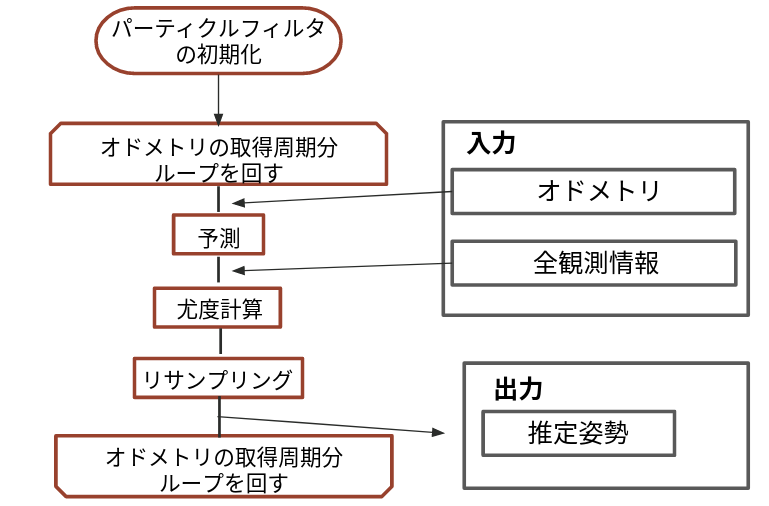
\includegraphics[width=1.0\linewidth]{figs/particle_filter_flow.png}
    \caption{パーティクルフィルタの流れ}
    \label{fig:particle_filter_flow}
  \end{center}
\end{figure}

\subsection{パーティクルフィルタの初期化}

まず、パーティクルの初期位置を$x_0$とする。


次に手持ちのマップから尤度場を求める。
尤度場は


\subsection{状態遷移モデルによる予測}

\subsection{尤度場を用いた、観測モデルによる尤度計算}

\subsection{リサンプリングによるパーティクルの更新}

\section{課題点}


\chapter{各パーティクルに観測範囲を可変にした未知障害物対策}
\section{はじめに}
この章では, 提案手法である, 各パーティクルに観測範囲を可変にした未知障害物の対策法について
説明する. 

\subsection{パーティクルに観測パターンを付与}
\subsection{尤度計算による観測パターンの評価}
\subsection{リサンプリング時にランダムな観測パターンを付与}
\subsection{尤度計算とリサンプリングによる観測パターンの収束}


